% lint-skip: 未完成ステータス（figure/table caption 未対応，人手チェック時に解消予定）
\documentclass[../../main.tex]{subfiles}
\begin{document}

\begin{flushright}
  \footnotesize\textit{【自動文字起こし・要確認】}
\end{flushright}

\noindent
{\bf [解答]}

\begin{enumerate}
  \item[(i)] 1辺の長さ1の辺が座標軸に平行な時.

    この正方形内部(周含む)の点 $(x, y)$ は, $\alpha, \beta \in \mathbb{R}$ として
    \[
      \begin{cases}
        \alpha \le x \le \alpha + 1 \\
        \beta \le y \le \beta + 1
      \end{cases}
    \]
    と書ける. この時, $\alpha \le m \le \alpha + 1$, $\beta \le n \le \beta + 1$ をみたす $m, n \in \mathbb{Z}$ が必ず存在するから, $(m, n)$ は正方形内部にある. 従って, 常に少なくとも1つの格子点を含む.

    \begin{figure}[htb]
      \centering
      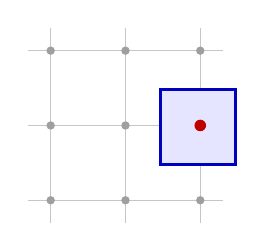
\begin{tikzpicture}[scale=0.95]
        \draw[step=1cm, gray!45, thin] (-0.3,-0.3) grid (2.3,2.3);
        \fill[blue!10] (1.47,0.48) rectangle (2.47,1.48);
        \draw[blue!75!black, very thick] (1.47,0.48) rectangle (2.47,1.48);
        \foreach \x in {0,1,2} {
          \foreach \y in {0,1,2} {
            \fill[gray!75] (\x,\y) circle (1.6pt);
          }
        }
        \fill[red!75!black] (2,1) circle (2.2pt);
      \end{tikzpicture}
      \caption{座標軸に平行な一辺 $1$ の正方形は格子点を含む。}
      \label{fig:1971_1_axis_aligned_square}
    \end{figure}

  \item[(ii)] 1辺の長さ $\sqrt{2}$ の時.

    1辺の長さ $\sqrt{2}$ の時, 右図から, 正方形の中心(対角線の交点)からの距離 $\dfrac{1}{2}$ の点は全て正方形内に含まれる. $\dots$ $\ast$

    又, 1辺1の正方形の4頂点となるような4格子点をもってくる. その内部 $A$ 内の任意の点は少なくとも1つの格子点からの距離が $\dfrac{\sqrt{2}}{2}$ 以下だから (対角線の長さ $\sqrt{2}$), $\ast$ より, 辺の長さ $\sqrt{2}$ の正方形は少なくとも1つの格子点を持つ.

    \begin{figure}[htb]
      \centering
      \begin{tikzpicture}[scale=1.5, >=stealth]
        \begin{scope}
          % Every orientation contains the same inscribed circle.
          \begin{scope}[rotate=18]
            \fill[blue!8] (-0.7071,-0.7071) rectangle (0.7071,0.7071);
            \draw[blue!75!black, very thick] (-0.7071,-0.7071) rectangle (0.7071,0.7071);
          \end{scope}
          \draw[teal!75!black, thick] (0,0) circle (0.7071);
          \fill[red!75!black] (0,0) circle (1.6pt);
          \node[below] at (0,-0.92) {一辺 $\sqrt{2}$};
        \end{scope}

        \begin{scope}[shift={(3.05,-0.5)}]
          \fill[gray!8] (0,0) rectangle (1,1);
          \draw[gray!75, thick] (0,0) rectangle (1,1);
          \foreach \x in {0,1} {
            \foreach \y in {0,1} {
              \fill[blue!75!black] (\x,\y) circle (1.7pt);
            }
          }
          \coordinate (A) at (0.5,0.5);
          \fill[red!75!black] (A) circle (1.6pt);
          \draw[red!75!black, dashed] (A) -- (1,1);
          \node[below left] at (A) {$A$};
          \node[right] at (0.77,0.76) {$\frac{\sqrt{2}}{2}$};
          \node[below] at (0.5,-0.18) {単位正方形};
        \end{scope}
      \end{tikzpicture}
      \caption{一辺 $\sqrt{2}$ の正方形の内接円と，単位正方形の中心から頂点までの距離。}
      \label{fig:1971_1_inscribed_circle}
    \end{figure}

    \noindent
    [\textbf{別}] (i)をつかうとお手軽. 径1の円に外接する座標軸に平行な辺を持つ正方形をもってきてもOK.
\end{enumerate}

\newpage

\end{document}
